\subsection{Exact points: the fate of the irrigation of one run}
The worked example of the guide (coarse loam, dose 10\,mm, April to October) drawn as one bar. Each segment is the difference between a flux of the irrigated run and the same flux of the rainfed run of the same soil and weather.
\begin{center}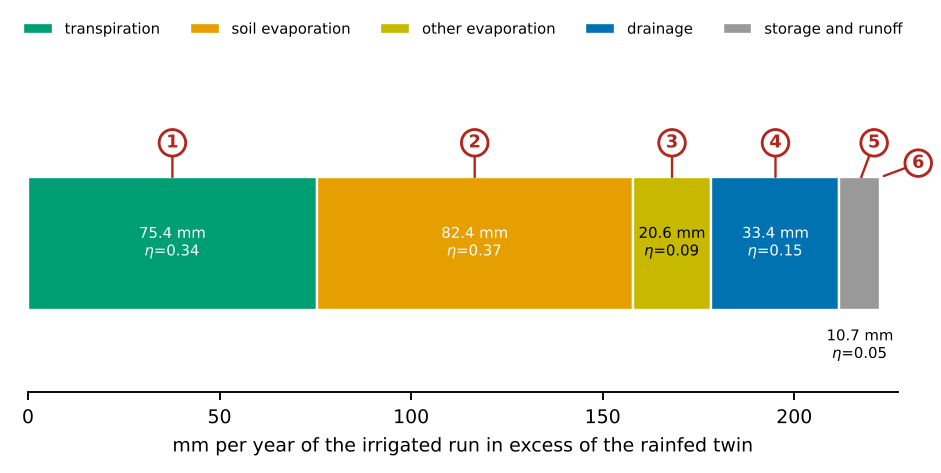
\includegraphics[width=0.92\textwidth]{../figures/paper4/ex_fate.png}\end{center}
\textbf{What the numbered labels point to, with the exact values.}
\begin{enumerate}[nosep,label=\protect\circled{\arabic*}]
\item Transpiration: 223.0 $-$ 147.6 = 75.4\,mm; $\eta_T=75.4/222.5=0.34$.
\item Soil evaporation: 82.4\,mm more than the rainfed twin; $\eta_{E_s}=0.37$, the largest share in this run because the surface is wetted every few days.
\item Other evaporation (interception, ponds, litter): 20.6\,mm; $\eta_{E_o}=0.09$.
\item Drainage below 1\,m: 39.5 $-$ 6.1 = 33.4\,mm; $\eta_D=0.15$.
\item The rest, 10.7\,mm, is the change of storage and runoff, obtained by difference so that the shares add to one.
\item The whole bar is the irrigation of the run, $I=222.5$\,mm a year: one bar is one irrigated millimetre scaled up.
\end{enumerate}
\textbf{How the exact points are obtained from the data.} The irrigated run is in experiment E10 and its rainfed twin in E0 (baseline of the same soil) of \nolinkurl{00_summary_all_simulations.csv.gz}; the columns used are \texttt{irrigation\_mm}, \texttt{transpiration\_mm}, \texttt{soil\_evap\_mm}, \texttt{ET\_mm} (other evaporation $=$ ET $-$ transpiration $-$ soil evaporation) and \texttt{drainage\_1m\_mm}; storage and runoff are $I-\Delta ET-\Delta D$. The article pools all irrigated runs of E10 of a soil (irrigation above 20\,mm a year) before dividing; the workbook sheet \texttt{EQ\_P4\_fate} repeats the pooled calculation with SUMIFS formulas.
